\documentclass{beamer}
\usepackage[utf8]{inputenc}
\usepackage[english,russian]{babel}
\usepackage{graphicx}
\usepackage{sidecap}

%beamer  theme's used to be here :)
\usetheme{mipt_beamer}

\title{Применение взаимодействующих нейронных сетей в криптографии}
\author{Ходаков Дмитрий.}
\date{March 14, 2014} %\today

\begin{document}
\frame{\titlepage}
\frame{\tableofcontents}
\section{Постановка задачи}
\subsection{Использование TPM}
\begin{frame}
\frametitle{Использование TPM}
Посмотрим, какова скорость схождения сети в зависимости от константы обучения.

\begin{center}
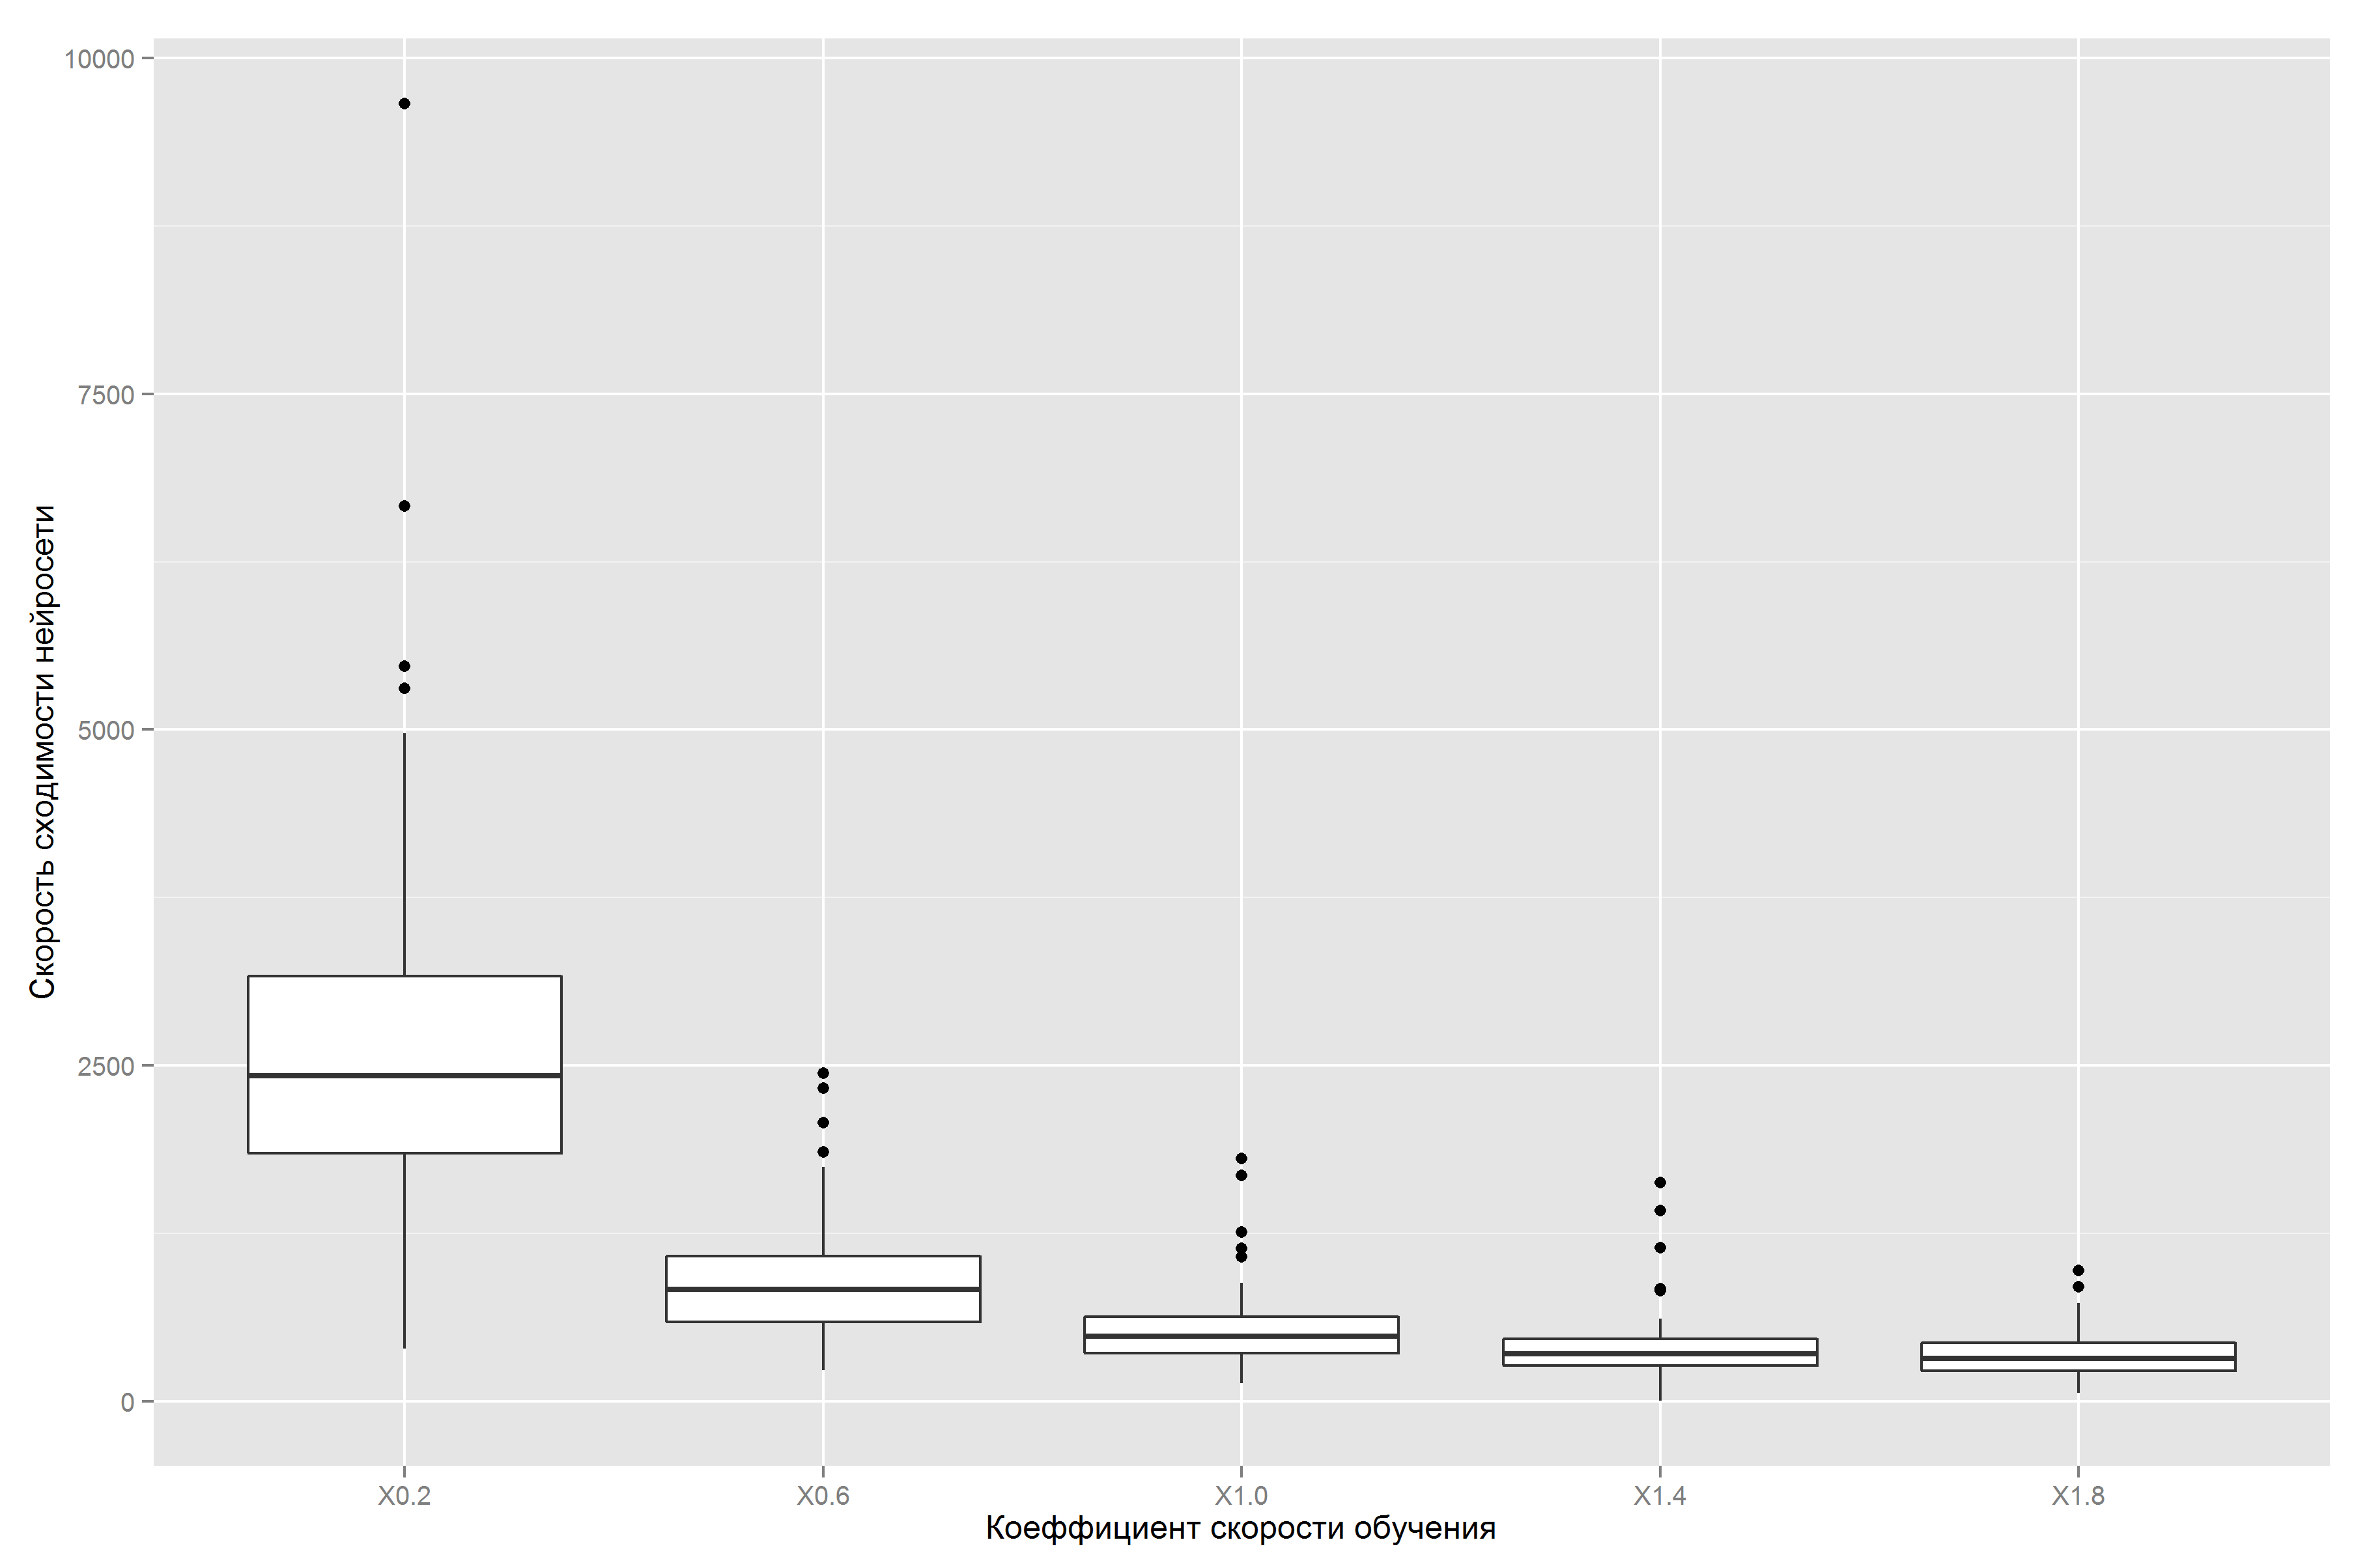
\includegraphics[width=5cm, height=5cm]{../../plots/eta_vs_speed.png}

\end{center}

\end{frame}

\end{document}